% Options for packages loaded elsewhere
\PassOptionsToPackage{unicode}{hyperref}
\PassOptionsToPackage{hyphens}{url}
\PassOptionsToPackage{dvipsnames,svgnames,x11names}{xcolor}
\PassOptionsToPackage{space}{xeCJK}
\documentclass[
  a4paper,
  10pt]{article}
\usepackage{xcolor}
\usepackage{amsmath,amssymb}
\setcounter{secnumdepth}{5}
\usepackage{iftex}
\ifPDFTeX
  \usepackage[T1]{fontenc}
  \usepackage[utf8]{inputenc}
  \usepackage{textcomp} % provide euro and other symbols
\else % if luatex or xetex
  \usepackage{unicode-math} % this also loads fontspec
  \defaultfontfeatures{Scale=MatchLowercase}
  \defaultfontfeatures[\rmfamily]{Ligatures=TeX,Scale=1}
\fi
\usepackage{lmodern}
\ifPDFTeX\else
  % xetex/luatex font selection
  \setmainfont[]{Times New Roman}
  \setmonofont[]{Menlo}
  \setmathfont[]{STIX Two Math}
  \ifXeTeX
    \usepackage{xeCJK}
    \setCJKmainfont[]{Songti SC}
  \fi
  \ifLuaTeX
    \usepackage[]{luatexja-fontspec}
    \setmainjfont[]{Songti SC}
  \fi
\fi
% Use upquote if available, for straight quotes in verbatim environments
\IfFileExists{upquote.sty}{\usepackage{upquote}}{}
\IfFileExists{microtype.sty}{% use microtype if available
  \usepackage[]{microtype}
  \UseMicrotypeSet[protrusion]{basicmath} % disable protrusion for tt fonts
}{}
\usepackage{longtable,booktabs,array}
\usepackage{caption}
\captionsetup[table]{skip=6pt}
\newcounter{none} % for unnumbered tables
\usepackage{calc} % for calculating minipage widths
% Correct order of tables after \paragraph or \subparagraph
\usepackage{etoolbox}
\makeatletter
\patchcmd\longtable{\par}{\if@noskipsec\mbox{}\fi\par}{}{}
\makeatother
% Allow footnotes in longtable head/foot
\IfFileExists{footnotehyper.sty}{\usepackage{footnotehyper}}{\usepackage{footnote}}
\makesavenoteenv{longtable}
\usepackage{graphicx}
\makeatletter
\newsavebox\pandoc@box
\newcommand*\pandocbounded[1]{% scales image to fit in text height/width
  \sbox\pandoc@box{#1}%
  \Gscale@div\@tempa{\textheight}{\dimexpr\ht\pandoc@box+\dp\pandoc@box\relax}%
  \Gscale@div\@tempb{\linewidth}{\wd\pandoc@box}%
  \ifdim\@tempb\p@<\@tempa\p@\let\@tempa\@tempb\fi% select the smaller of both
  \ifdim\@tempa\p@<\p@\scalebox{\@tempa}{\usebox\pandoc@box}%
  \else\usebox{\pandoc@box}%
  \fi%
}
% Set default figure placement to htbp
\def\fps@figure{htbp}
\makeatother
\setlength{\emergencystretch}{3em} % prevent overfull lines
\providecommand{\tightlist}{%
  \setlength{\itemsep}{0pt}\setlength{\parskip}{0pt}}
\usepackage[a4paper,top=24mm,bottom=25mm,left=23mm,right=23mm,headheight=15pt]{geometry}
\usepackage{amsmath,amssymb,mathtools,bm}
\usepackage{booktabs,longtable,array}
\usepackage{graphicx}
\usepackage{float}
\usepackage{caption}
\usepackage{enumitem}
\usepackage{fancyhdr}
\usepackage{titlesec}
\usepackage{mdframed}
\usepackage{xcolor}
\usepackage{xurl}
\usepackage{hyperref}
\graphicspath{{../../}}

\definecolor{PaperBlue}{HTML}{000000}
\definecolor{PaperRule}{HTML}{B7C6D5}
\definecolor{PaperShade}{HTML}{F4F7FA}
\definecolor{PaperText}{HTML}{000000}

\hypersetup{
  colorlinks=true,
  linkcolor=PaperBlue,
  urlcolor=PaperBlue,
  citecolor=PaperBlue,
  pdfborder={0 0 0}
}

\color{PaperText}
\linespread{1.08}
\setlength{\parindent}{1.5em}
\setlength{\parskip}{0.25em}
\setlength{\emergencystretch}{3em}
\setlist{itemsep=0.2em,topsep=0.45em}
\setcounter{secnumdepth}{3}
\setcounter{tocdepth}{3}

\titleformat{\section}
  {\Large\bfseries\color{PaperBlue}}
  {\thesection}{0.7em}{}
\titleformat{\subsection}
  {\large\bfseries\color{PaperText}}
  {\thesubsection}{0.65em}{}
\titleformat{\subsubsection}
  {\normalsize\bfseries\color{PaperText}}
  {\thesubsubsection}{0.6em}{}
\titlespacing*{\section}{0pt}{2.2ex plus 0.5ex}{0.9ex}
\titlespacing*{\subsection}{0pt}{1.8ex plus 0.4ex}{0.7ex}
\titlespacing*{\subsubsection}{0pt}{1.5ex plus 0.3ex}{0.5ex}

\captionsetup{
  font=small,
  labelfont=bf,
  textfont=it,
  justification=centering,
  skip=6pt
}

\pagestyle{fancy}
\fancyhf{}
\fancyhead[L]{\small\nouppercase{\leftmark}}
\fancyhead[R]{\small Selene's Blog}
\fancyfoot[C]{\small\thepage}
\renewcommand{\headrulewidth}{0.4pt}
\renewcommand{\footrulewidth}{0pt}
\fancypagestyle{plain}{
  \fancyhf{}
  \fancyhead[R]{\small Selene's Blog}
  \fancyfoot[C]{\small\thepage}
  \renewcommand{\headrulewidth}{0.4pt}
}

\renewenvironment{quote}
  {\begin{mdframed}[
      linewidth=0.7pt,
      linecolor=PaperRule,
      backgroundcolor=PaperShade,
      leftline=true,
      rightline=false,
      topline=false,
      bottomline=false,
      innerleftmargin=10pt,
      innerrightmargin=8pt,
      innertopmargin=7pt,
      innerbottommargin=7pt,
      skipabove=8pt,
      skipbelow=10pt
    ]\itshape}
  {\end{mdframed}}

\newenvironment{theorembox}[1]
  {\par\medskip\noindent\textbf{Theorem (#1).}\quad}
  {\par\medskip}

\newenvironment{lemmabox}[1]
  {\par\medskip\noindent\textbf{Lemma #1.}\quad}
  {\par\medskip}

\newenvironment{proofbox}
  {\par\medskip\noindent\textit{Proof.}\quad}
  {\hfill$\square$\par\medskip}

\AtBeginDocument{\allowdisplaybreaks[2]}
\usepackage{bookmark}
\IfFileExists{xurl.sty}{\usepackage{xurl}}{} % add URL line breaks if available
\urlstyle{same}
% fallback for those not using the hyperref driver hyperxmp:
\makeatletter
\@ifundefined{xmpquote}{\newcommand{\xmpquote}[1]{#1}}{}
\makeatother
\hypersetup{
  pdftitle={CS224N \textbar{} Neural Networks and Backpropagation},
  pdfauthor={Selene},
  colorlinks=true,
  linkcolor={black},
  filecolor={Maroon},
  citecolor={Blue},
  urlcolor={black},
  pdfcreator={LaTeX via pandoc}}

\title{CS224N \textbar{} Neural Networks and Backpropagation}
\author{Selene}
\date{August 10, 2026}

\begin{document}
\maketitle

\section{Neural Networks and
Backpropagation}\label{neural-networks-and-backpropagation}

\subsection{Neural Networks}\label{neural-networks}

\subsubsection{A Single Neuron}\label{a-single-neuron}

A neuron receives \(n\) inputs and produces one output. Different
neurons produce different outputs because they have different
parameters. A common example is the sigmoid logistic unit. It receives
an \(n\)-dimensional input vector \(x\) and produces an activation value
\(a\). The neuron also has an \(n\)-dimensional weight vector \(w\) and
a scalar bias \(b\). Its output is

\[
a=\frac{1}{1+\exp\left(-\left(w^\top x+b\right)\right)}.
\]

\subsubsection{A Single Layer of
Neurons}\label{a-single-layer-of-neurons}

Now extend this idea to multiple neurons. Suppose their weight vectors
are \(\{w^{(1)},w^{(2)},\dots,w^{(m)}\}\), their biases are
\(\{b_1,\dots,b_m\}\), and their corresponding activations are
\(\{a_1,\dots,a_m\}\):

\[
a_1=\frac{1}{1+\exp\left(-\left(w^{(1)\top}x+b_1\right)\right)},
\]

\[
\vdots
\]

\[
a_m=\frac{1}{1+\exp\left(-\left(w^{(m)\top}x+b_m\right)\right)}.
\]

To simplify the notation and make more complex networks easier to
describe, define

\[
\sigma(z)=
\begin{bmatrix}
\dfrac{1}{1+\exp(-z_1)}\\
\vdots\\
\dfrac{1}{1+\exp(-z_m)}
\end{bmatrix},
\qquad
b=
\begin{bmatrix}
b_1\\
\vdots\\
b_m
\end{bmatrix}
\in\mathbb{R}^m,
\]

and

\[
W=
\begin{bmatrix}
w^{(1)\top}\\
\vdots\\
w^{(m)\top}
\end{bmatrix}
\in\mathbb{R}^{m\times n}.
\]

The pre-activation vector is therefore

\[
z=Wx+b,
\]

and the vector of sigmoid activations can be written as

\[
a=
\begin{bmatrix}
a_1\\
\vdots\\
a_m
\end{bmatrix}
=\sigma(z)=\sigma(Wx+b).
\]

\subsubsection{Feedforward Computation}\label{feedforward-computation}

The feedforward computation of a neural network is

\[
a=f(Wx+b),
\]

where \(x\) is the input, \(W\) and \(b\) are parameters, \(f\) is an
activation function, and \(a\) is the hidden-layer activation. The
output score is then computed from the hidden layer:

\[
s=U^\top a=U^\top f(Wx+b).
\]

The hidden layer applies a nonlinear transformation to extract
combinations of input features, allowing the model to learn more complex
relationships.

\subsubsection{Maximum-Margin Objective}\label{maximum-margin-objective}

Like most machine-learning models, a neural network needs an
optimization objective. A maximum-margin objective encourages the score
of a correctly labeled example to exceed that of an incorrectly labeled
example. Let \(s\) denote the score of the correct example and \(s_c\)
the score of an incorrect example, where

\[
s_c=U^\top f(Wx_c+b),
\qquad
s=U^\top f(Wx+b).
\]

The objective should maximize \(s-s_c\), or equivalently minimize
\(s_c-s\). If we only considered the case \(s_c>s\), the objective would
be \(\operatorname{minimize} J=\max(s_c-s,0)\). However, we want the
correct example to score at least a positive margin \(\Delta\) above the
incorrect example. The objective therefore becomes

\[
\operatorname{minimize}\quad
J=\max(\Delta+s_c-s,0).
\]

\subsubsection{Backpropagation}\label{backpropagation}

This section discusses how to train the model parameters when the cost
\(J\) is positive. If the cost is zero, no parameter update is needed.
We usually update parameters with gradient descent, so we need the
gradient of the loss with respect to every parameter:

\[
\theta^{(t+1)}
=\theta^{(t)}
-\alpha\nabla_{\theta^{(t)}}J.
\]

The chain rule allows us to calculate the loss gradient for any
parameter used in the feedforward computation.

\begin{figure}
\centering
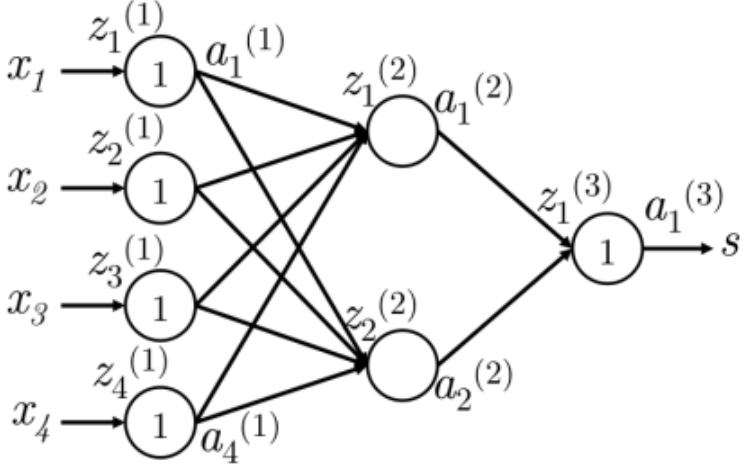
\includegraphics[width=0.8\linewidth,height=\textheight,keepaspectratio,alt={A three-layer neural network and its feedforward connections}]{assets/img/posts/neural-networks-and-backpropagation/network-architecture.png}
\caption{A three-layer neural network and its feedforward connections}
\end{figure}

\textbf{Notation}

{\def\LTcaptype{none} % do not increment counter
\begin{longtable}[]{@{}
  >{\raggedright\arraybackslash}p{(\linewidth - 2\tabcolsep) * \real{0.5000}}
  >{\raggedright\arraybackslash}p{(\linewidth - 2\tabcolsep) * \real{0.5000}}@{}}
\toprule\noalign{}
\begin{minipage}[b]{\linewidth}\raggedright
Symbol
\end{minipage} & \begin{minipage}[b]{\linewidth}\raggedright
Meaning
\end{minipage} \\
\midrule\noalign{}
\endhead
\bottomrule\noalign{}
\endlastfoot
\(x_i\) & The \(i\)-th input to the neural network \\
\(s\) & The output of the neural network \\
\(z_j^{(k)}\) & The scalar input received by neuron \(j\) in layer
\(k\) \\
\(a_j^{(k)}\) & The activation output produced by neuron \(j\) in layer
\(k\) \\
\(\delta_j^{(k)}\) & The error computed at \(z_j^{(k)}\) and propagated
backward \\
\(W^{(k)}\) & The weight matrix mapping the outputs of layer \(k\) to
the inputs of layer \(k+1\) \\
\end{longtable}
}

The first layer is the input layer, so

\[
x_j=z_j^{(1)}=a_j^{(1)}.
\]

Using the notation introduced earlier,

\[
W^{(1)}=W,
\qquad
W^{(2)}=U.
\]

We now begin the derivation. Assume that \(J=1+s_c-s>0\), and consider
updating the parameter \(W_{14}^{(1)}\). This parameter affects only the
input \(z_1^{(2)}\) of the first hidden-layer neuron, which in turn
affects \(a_1^{(2)}\). The gradient therefore propagates backward only
along paths influenced by this parameter.

From the maximum-margin loss,

\[
\frac{\partial J}{\partial s}=-1,
\qquad
\frac{\partial J}{\partial s_c}=1.
\]

Consider the effect of the first-layer weight \(W_{ij}^{(1)}\) on the
output \(s\). By the chain rule,

\[
\begin{aligned}
\frac{\partial s}{\partial W_{ij}^{(1)}}
&=W_i^{(2)}\frac{\partial a_i^{(2)}}{\partial W_{ij}^{(1)}}\\
&=W_i^{(2)}
\frac{\partial a_i^{(2)}}{\partial z_i^{(2)}}
\frac{\partial z_i^{(2)}}{\partial W_{ij}^{(1)}}\\
&=W_i^{(2)}f'\left(z_i^{(2)}\right)
\frac{\partial z_i^{(2)}}{\partial W_{ij}^{(1)}}.
\end{aligned}
\]

The input to neuron \(i\) in the second layer is

\[
z_i^{(2)}
=b_i^{(1)}+\sum_k a_k^{(1)}W_{ik}^{(1)},
\]

so

\[
\frac{\partial z_i^{(2)}}{\partial W_{ij}^{(1)}}
=a_j^{(1)}.
\]

Substitution gives

\[
\frac{\partial s}{\partial W_{ij}^{(1)}}
=W_i^{(2)}f'\left(z_i^{(2)}\right)a_j^{(1)}.
\]

Define the backpropagated error of neuron \(i\) in the second layer as

\[
\delta_i^{(2)}
=W_i^{(2)}f'\left(z_i^{(2)}\right).
\]

Then

\[
\frac{\partial s}{\partial W_{ij}^{(1)}}
=\delta_i^{(2)}a_j^{(1)}.
\]

Here, \(\delta_i^{(2)}\) is the backward error at neuron \(i\) in layer
\(2\), while \(a_j^{(1)}\) is the activation from the previous layer
that enters the weight \(W_{ij}^{(1)}\). In short:

\[
\text{weight gradient}
=\text{backward error}\times\text{forward input}.
\]

For example, \(W_{14}^{(1)}\) affects only the first hidden-layer
neuron, so the error propagates backward along the corresponding path:

\begin{enumerate}
\def\labelenumi{\arabic{enumi}.}
\item
  Start at the output \(a_1^{(3)}\) and propagate an error signal of
  magnitude \(1\) backward.
\item
  As the error passes through \(z_1^{(3)}\to a_1^{(3)}\), multiply it by
  the local gradient. The local gradient here is \(1\), so

  \[
  \delta_1^{(3)}=1.
  \]
\item
  The error continues to the previous layer. It is distributed to
  \(a_1^{(2)}\) through the weight \(W_1^{(2)}\), giving
  \(W_1^{(2)}\delta_1^{(3)}=W_1^{(2)}\).
\item
  As the error passes through \(z_1^{(2)}\to a_1^{(2)}\), multiply it by
  the local derivative \(f'\left(z_1^{(2)}\right)\):

  \[
  \delta_1^{(2)}
  =f'\left(z_1^{(2)}\right)W_1^{(2)}.
  \]
\item
  Finally, \(W_{14}^{(1)}\) receives \(a_4^{(1)}\) during the forward
  pass, so its gradient is

  \[
  \frac{\partial s}{\partial W_{14}^{(1)}}
  =\delta_1^{(2)}a_4^{(1)}
  =a_4^{(1)}f'\left(z_1^{(2)}\right)W_1^{(2)}.
  \]
\end{enumerate}

\textbf{Bias Updates}

A bias can be viewed as a special weight whose input is always \(1\).
Therefore, the bias gradient of neuron \(i\) in layer \(k\) is its
backpropagated error:

\[
\frac{\partial J}{\partial b_i^{(k)}}
=\delta_i^{(k)}.
\]

For example, the gradient of \(b_1^{(1)}\) is

\[
\frac{\partial J}{\partial b_1^{(1)}}
=\delta_1^{(2)}
=f'\left(z_1^{(2)}\right)W_1^{(2)}.
\]

\textbf{General Procedure for Propagating \(\delta^{(k)}\) to
\(\delta^{(k-1)}\)}

\begin{enumerate}
\def\labelenumi{\arabic{enumi}.}
\item
  The error \(\delta_i^{(k)}\) at neuron \(i\) in layer \(k\) propagates
  toward the preceding layer along the weight \(W_{ij}^{(k-1)}\).

  \begin{figure}
  \centering
  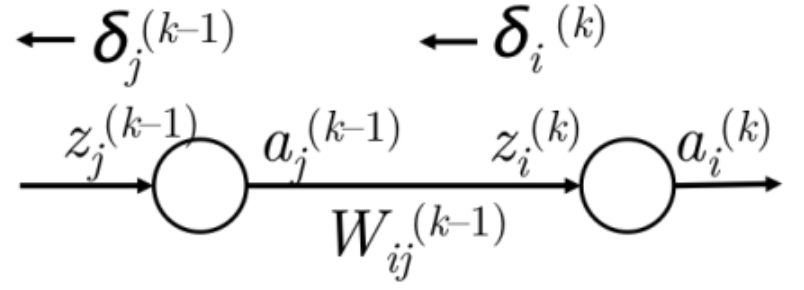
\includegraphics[width=0.85\linewidth,height=\textheight,keepaspectratio,alt={An error signal propagating backward through a weighted connection}]{assets/img/posts/neural-networks-and-backpropagation/backpropagation-connection.png}
  \caption{An error signal propagating backward through a weighted
  connection}
  \end{figure}
\item
  Along one connection to neuron \(j\) in layer \(k-1\), the path
  contributes the error \(\delta_i^{(k)}W_{ij}^{(k-1)}\).
\item
  Because neuron \(j\) in layer \(k-1\) is usually connected to several
  neurons in the next layer, sum the errors from all paths:

  \[
  \sum_i\delta_i^{(k)}W_{ij}^{(k-1)}.
  \]
\item
  After obtaining the total error, multiply it by the local derivative
  \(f'\left(z_j^{(k-1)}\right)\) of that neuron's activation function.
\item
  The error at neuron \(j\) in layer \(k-1\) is therefore

  \[
  \delta_j^{(k-1)}
  =f'\left(z_j^{(k-1)}\right)
  \sum_i\delta_i^{(k)}W_{ij}^{(k-1)}.
  \]
\end{enumerate}

\subsubsection{Training with Backpropagation: Vectorized
Form}\label{training-with-backpropagation-vectorized-form}

So far, we have discussed how to compute the gradient of one parameter.
We now generalize the method so that an entire weight matrix can be
updated at once.

For a parameter \(W_{ij}^{(k)}\), the gradient derived above is
\(\delta_i^{(k+1)}a_j^{(k)}\). Therefore, the gradient of the entire
matrix \(W^{(k)}\) is

\[
\nabla W^{(k)}=
\begin{bmatrix}
\delta_1^{(k+1)}a_1^{(k)} & \delta_1^{(k+1)}a_2^{(k)} & \cdots\\
\delta_2^{(k+1)}a_1^{(k)} & \delta_2^{(k+1)}a_2^{(k)} & \cdots\\
\vdots & \vdots & \ddots
\end{bmatrix}
=\delta^{(k+1)}a^{(k)\top}.
\]

Thus, the matrix gradient is the outer product of the error vector
entering the matrix during backpropagation and the activation vector
that passed forward through the matrix. The vectorized error recurrence
is

\[
\delta^{(k)}
=f'\left(z^{(k)}\right)
\circ\left(W^{(k)\top}\delta^{(k+1)}\right),
\]

where \(\circ\) denotes element-wise multiplication.

\subsection{Practical Techniques for Neural
Networks}\label{practical-techniques-for-neural-networks}

\subsubsection{Regularization}\label{regularization}

Like many machine-learning models, neural networks can easily overfit.
One common remedy is to add an \(L_2\) regularization penalty to the
loss \(J\):

\[
J_R
=J+\lambda\sum_{i=1}^{L}
\left\lVert W^{(i)}\right\rVert_F^2.
\]

Here, \(\left\lVert W^{(i)}\right\rVert_F\) is the Frobenius norm of
\(W^{(i)}\), and \(\lambda\) is a hyperparameter controlling the
strength of the penalty relative to the original loss. Because the
objective minimizes \(J_R\), regularization penalizes excessively large
weights while optimizing the loss. The quadratic nature of the penalty
reduces the model's flexibility and helps alleviate overfitting.

\begin{quote}
The Frobenius norm of a matrix \(U\) is
\(\left\lVert U\right\rVert_F=\sqrt{\sum_i\sum_j U_{ij}^2}\).
\end{quote}

This constraint can also be interpreted as a Bayesian prior stating that
the optimal weights should be close to zero. How close they should be
depends on \(\lambda\), so choosing an appropriate value requires
hyperparameter tuning. If \(\lambda\) is too large, most weights are
forced close to zero and the model cannot learn meaningful information
from the training data. It will usually perform poorly on the training,
validation, and test sets. If \(\lambda\) is too small, the model may
overfit again.

Bias terms are not normally regularized because a bias \(b\) controls an
overall translation of the model and does not substantially increase its
complexity, whereas a weight \(w\) determines sensitivity to the input
and is more likely to contribute to overfitting.

\subsubsection{Dropout}\label{dropout}

\textbf{Dropout} is a powerful regularization technique with a simple
idea: during each forward and backward pass in training, independently
discard each neuron with probability \(1-p\), or equivalently retain it
with probability \(p\). At test time, use the complete network to
compute predictions. Dropout encourages the network to learn more robust
representations and can reduce overfitting. It can also be viewed as
training an exponential number of smaller subnetworks and approximately
averaging their predictions.

In practice, for each layer output \(h\), retain each activation with
probability \(p\) and otherwise set it to zero. During backpropagation,
gradients pass only through neurons retained in the forward pass.

A key detail is that the expected scale of the activations should remain
approximately the same during training and testing. The most common
implementation is \textbf{inverted dropout}, which divides retained
activations by \(p\) during training and requires no scaling at test
time. Alternatively, if activations are not scaled during training,
multiply them by \(p\) at test time.

\subsubsection{Neuron Units}\label{neuron-units}

The neural networks discussed so far use sigmoid neurons to introduce
nonlinearity. In many applications, however, other activation functions
work better. The following functions and their derivatives are common
alternatives.

\textbf{Sigmoid.} The sigmoid activation is

\[
\sigma(z)=\frac{1}{1+\exp(-z)}.
\]

Its derivative is

\[
\sigma'(z)
=\frac{\exp(-z)}{\left(1+\exp(-z)\right)^2}
=\sigma(z)\left(1-\sigma(z)\right).
\]

\begin{figure}
\centering
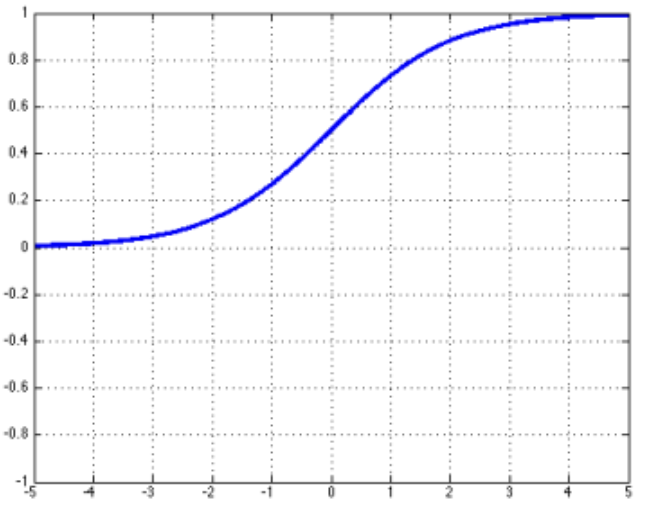
\includegraphics[width=0.46\linewidth,height=\textheight,keepaspectratio,alt={The sigmoid activation function}]{assets/img/posts/neural-networks-and-backpropagation/sigmoid.png}
\caption{The sigmoid activation function}
\end{figure}

\textbf{Tanh.} The hyperbolic tangent is an alternative to the sigmoid
and often converges faster in practice. Tanh outputs values between
\(-1\) and \(1\), whereas sigmoid outputs values between \(0\) and
\(1\):

\[
\tanh(z)
=\frac{\exp(z)-\exp(-z)}{\exp(z)+\exp(-z)}
=2\sigma(2z)-1,
\qquad
\tanh(z)\in(-1,1).
\]

Its derivative is

\[
\tanh'(z)
=1-\left(
\frac{\exp(z)-\exp(-z)}{\exp(z)+\exp(-z)}
\right)^2
=1-\tanh^2(z).
\]

\begin{figure}
\centering
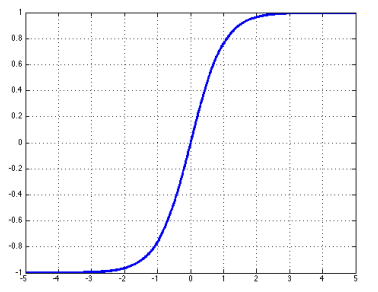
\includegraphics[width=0.48\linewidth,height=\textheight,keepaspectratio,alt={The tanh activation function}]{assets/img/posts/neural-networks-and-backpropagation/tanh.png}
\caption{The tanh activation function}
\end{figure}

\textbf{Hard Tanh.} Hard Tanh is sometimes used in place of Tanh because
it is less expensive to compute, although it saturates when
\(\lvert z\rvert>1\):

\[
\operatorname{hardtanh}(z)=
\begin{cases}
-1, & z<-1,\\
z, & -1\le z\le 1,\\
1, & z>1.
\end{cases}
\]

Its derivative is

\[
\operatorname{hardtanh}'(z)=
\begin{cases}
1, & -1<z<1,\\
0, & \text{otherwise}.
\end{cases}
\]

\begin{figure}
\centering
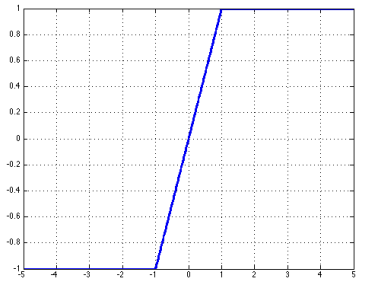
\includegraphics[width=0.48\linewidth,height=\textheight,keepaspectratio,alt={The Hard Tanh activation function}]{assets/img/posts/neural-networks-and-backpropagation/hard-tanh.png}
\caption{The Hard Tanh activation function}
\end{figure}

\textbf{Softsign.} Softsign is another nonlinear alternative to Tanh.
Its tails approach saturation more gradually than those of Tanh:

\[
\operatorname{softsign}(z)
=\frac{z}{1+\lvert z\rvert}.
\]

Its derivative is

\[
\operatorname{softsign}'(z)
=\frac{1}{\left(1+\lvert z\rvert\right)^2}.
\]

\begin{figure}
\centering
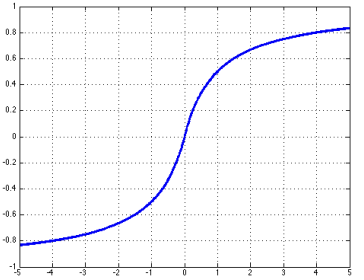
\includegraphics[width=0.48\linewidth,height=\textheight,keepaspectratio,alt={The Softsign activation function}]{assets/img/posts/neural-networks-and-backpropagation/softsign.png}
\caption{The Softsign activation function}
\end{figure}

\textbf{ReLU.} The rectified linear unit is a widely used activation
function. It does not saturate for large positive values of \(z\) and
has achieved strong results in computer-vision applications:

\[
\operatorname{ReLU}(z)=\max(z,0).
\]

Its derivative is the piecewise function

\[
\operatorname{ReLU}'(z)=
\begin{cases}
1, & z>0,\\
0, & z<0.
\end{cases}
\]

At \(z=0\), a subgradient such as \(0\) is chosen by convention.

\begin{figure}
\centering
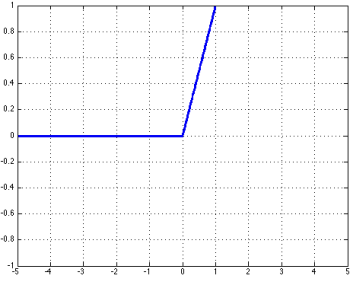
\includegraphics[width=0.48\linewidth,height=\textheight,keepaspectratio,alt={The ReLU activation function}]{assets/img/posts/neural-networks-and-backpropagation/relu.png}
\caption{The ReLU activation function}
\end{figure}

\textbf{Leaky ReLU.} A conventional ReLU does not propagate an error
signal when \(z<0\). Leaky ReLU modifies it so that a small gradient can
still propagate when \(z\) is negative:

\[
\operatorname{LeakyReLU}(z)
=\max(z,kz),
\qquad
0<k<1.
\]

Its derivative is

\[
\operatorname{LeakyReLU}'(z)=
\begin{cases}
1, & z>0,\\
k, & z<0.
\end{cases}
\]

\begin{figure}
\centering
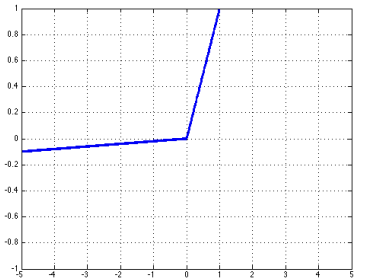
\includegraphics[width=0.48\linewidth,height=\textheight,keepaspectratio,alt={The Leaky ReLU activation function}]{assets/img/posts/neural-networks-and-backpropagation/leaky-relu.png}
\caption{The Leaky ReLU activation function}
\end{figure}

\subsubsection{Data Preprocessing}\label{data-preprocessing}

As with other machine-learning models, basic data preprocessing is
essential for obtaining reasonable performance on the target task.

\textbf{Mean subtraction.} Given an input dataset \(X\), subtract the
mean feature vector from every example so that the data is centered at
zero. In practice, compute the mean using only the training set, then
subtract that same mean from the training, validation, and test sets.

\textbf{Normalization.} Another common technique, though sometimes used
less often than mean subtraction, is to scale every input feature
dimension to a similar range. This is useful because input features are
often measured in different units, while initially we usually want to
treat all features as equally important. Compute each feature's standard
deviation on the training set, then divide that feature by the
corresponding value across the training, validation, and test sets.

\textbf{Whitening.} Whitening is less common than mean subtraction
followed by normalization. It transforms the data so that its covariance
matrix is the identity: the features become uncorrelated and each has
variance \(1\). First subtract the mean from the data to obtain \(X'\).
Next, compute the singular value decomposition of \(X'\), obtaining
\(U\), \(S\), and \(V\). Project \(X'\) into the basis defined by the
columns of \(U\), then divide each resulting dimension by its
corresponding singular value in \(S\). If a singular value is zero,
divide by a small positive value instead for numerical stability.

\end{document}
